\documentclass[dvipsnames,pdf,9pt]{beamer}
\usepackage{listings,graphicx,verbatimbox,hyperref}
%\usepackage{bibentry}
% \usepackage[customcolors,shade]{hf-tikz}
% \usepackage{tikz}
\usepackage{amsmath}
\usepackage{xcolor}

\newcommand*{\colorboxed}{}
\def\colorboxed#1#{%
  \colorboxedAux{#1}%
}
\newcommand*{\colorboxedAux}[3]{%
  % #1: optional argument for color model
  % #2: color specification
  % #3: formula
  \begingroup
  \colorlet{cb@saved}{.}%
  \color#1{#2}%
  \boxed{%
    \color{cb@saved}%
    #3%
  }%
  \endgroup
}

\newcommand{\N}{\mathbb{N}}
\newcommand{\Z}{\mathbb{Z}}
\newcommand{\Q}{\mathbb{Q}}
\newcommand{\R}{\mathbb{R}}
\newcommand{\C}{\mathbb{C}}
\newcommand{\norm}[1]{\left\lVert#1\right\rVert}
\newcommand{\ceil}[1]{\lceil#1\rceil}
\newcommand{\ov}{\overline}
\newcommand{\cleq}{\preccurlyeq}
\newcommand{\cgeq}{\succcurlyeq}
\newcommand{\bdy}{\textbf{\text{Bdy}}}
\newcommand{\trace}{\text{trace}}
\newcommand{\dom}{\textbf{dom}}
\newcommand{\expec}{\mathbb{E}}
\newcommand{\bigO}{\mathcal{O}}
\newcommand{\tr}{\text{tr}}
\newcommand{\<}{\langle}
\renewcommand{\>}{\rangle}
\newcommand*\oldmacro{}%
\let\oldmacro\insertshorttitle%
% \renewcommand*\insertshorttitle{%
% \oldmacro\hfill%
% \insertframenumber\,/\,\inserttotalframenumber}
\DeclareMathOperator*{\argmax}{arg\,max}
\DeclareMathOperator*{\argmin}{arg\,min}

% use the below command to restart numbering in an enumeration, using alphabetics
% \setbeamertemplate{enumerate item}{(\alph{enumi})}
% \setbeamertemplate{enumerate subitem}{(\roman{enumii})}
\setbeamertemplate{navigation symbols}{}

% \usetheme{Warsaw}

\usepackage[style=nature]{biblatex}
\addbibresource{refs.bib}

\DeclareCiteCommand{\footcite}[\mkbibfootnote]
  {\usebibmacro{prenote}}
  {\printnames[family-given]{labelname}%
   \hspace{1mm} \printfield{journaltitle}%
   \hspace{1mm} \printfield{year}}
  {\addsemicolon\space}
  {\usebibmacro{postnote}}

\setbeamertemplate{footline}
{
  \leavevmode%
  \hbox{%
    \begin{beamercolorbox}[wd=.3\paperwidth,ht=2.25ex,dp=1ex,center]{author in head/foot}%
      \usebeamerfont{author in head/foot}\insertshortauthor
    \end{beamercolorbox}%
    \begin{beamercolorbox}[wd=.7\paperwidth,ht=2.25ex,dp=1ex,center]{title in head/foot}%
      \usebeamerfont{title in head/foot}\insertshorttitle\hspace*{3em}
      \insertframenumber{} / \inserttotalframenumber\hspace*{1ex}
    \end{beamercolorbox}}%
  \vskip0pt%
}

\setbeamersize{text margin left=5mm,text margin right=7mm}

\usepackage{caption}
\title{Introduction to Parallelism \& Parallelism on HPC}
\subtitle{Examples in Julia and Python}
\author[cmhyett@math.arizona.edu]{Criston Hyett}

\def\bb_{f}

\begin{document}
\graphicspath{{./figures/}}
%%%%%%%%%%%%%%%%%%%%%%%%%%%%%%%%%%%%%%%%%%%%%%%%%%%%%%%%%%%%%%%%%%%%%%%%%%%%% 
\begin{frame}
  \titlepage
\end{frame}
%%%%%%%%%%%%%%%%%%%%%%%%%%%%%%%%%%%%%%%%%%%%%%%%%%%%%%%%%%%%%%%%%%%%%%%%%%%%% 

%%%%%%%%%%%%%%%%%%%%%%%%%%%%%%%%%%%%%%%%%%%%%%%%%%%%%%%%%%%%%%%%%%%%%%%%%%%%% 
\begin{frame}{What is parallelism?}
  \begin{itemize}
  \item The common idea of \textbf{divide and conquer}
  \item Works extremely well in many relevant scenarios
    \begin{itemize}
    \item Large dimension linear algebra, (i.e. ML)
    \item Monte Carlo
    \item Ordinary/Partial/Stochastic Differential equations (big linear algebra + Monte Carlo)
    \end{itemize}
  \item Not a panacea!
    \begin{itemize}
    \item Inefficient code can be inefficient \textit{and} consume plenty of cpu-hours on the HPC
    \end{itemize}
  \end{itemize}
\end{frame}
%%%%%%%%%%%%%%%%%%%%%%%%%%%%%%%%%%%%%%%%%%%%%%%%%%%%%%%%%%%%%%%%%%%%%%%%%%%%% 

%%%%%%%%%%%%%%%%%%%%%%%%%%%%%%%%%%%%%%%%%%%%%%%%%%%%%%%%%%%%%%%%%%%%%%%%%%%%% 
\begin{frame}{When should you care?}
  \only<1->{
    \begin{itemize}
    \item When the benefits outweigh the costs!
    \item Costs
      \begin{itemize}
      \item \textbf{Human costs:} Coding, debugging, refactoring
      \item \textbf{Computational Costs:} parallelism requires coordination between threads, and/or nodes. When this coordination is required often, or significant data is passing between threads, parallel benefits may be outweighed.
      \end{itemize}
    \item Benefits
      \begin{itemize}
      \item \textbf{Computation speed}
      \item \textbf{Smaller memory overheads per thread}
      \item Process independence
      \end{itemize}
    \end{itemize}
  }
  \only<2>{
    \begin{centering}
      \textbf{Many of the costs are mitigated by modern languages providing thread-safe, optimized libraries.}
    \end{centering}
  }
\end{frame}
%%%%%%%%%%%%%%%%%%%%%%%%%%%%%%%%%%%%%%%%%%%%%%%%%%%%%%%%%%%%%%%%%%%%%%%%%%%%% 

%%%%%%%%%%%%%%%%%%%%%%%%%%%%%%%%%%%%%%%%%%%%%%%%%%%%%%%%%%%%%%%%%%%%%%%%%%%%% 
\begin{frame}[fragile]{Parallel paradigms: CPU}
  \begin{figure}
    \centering
    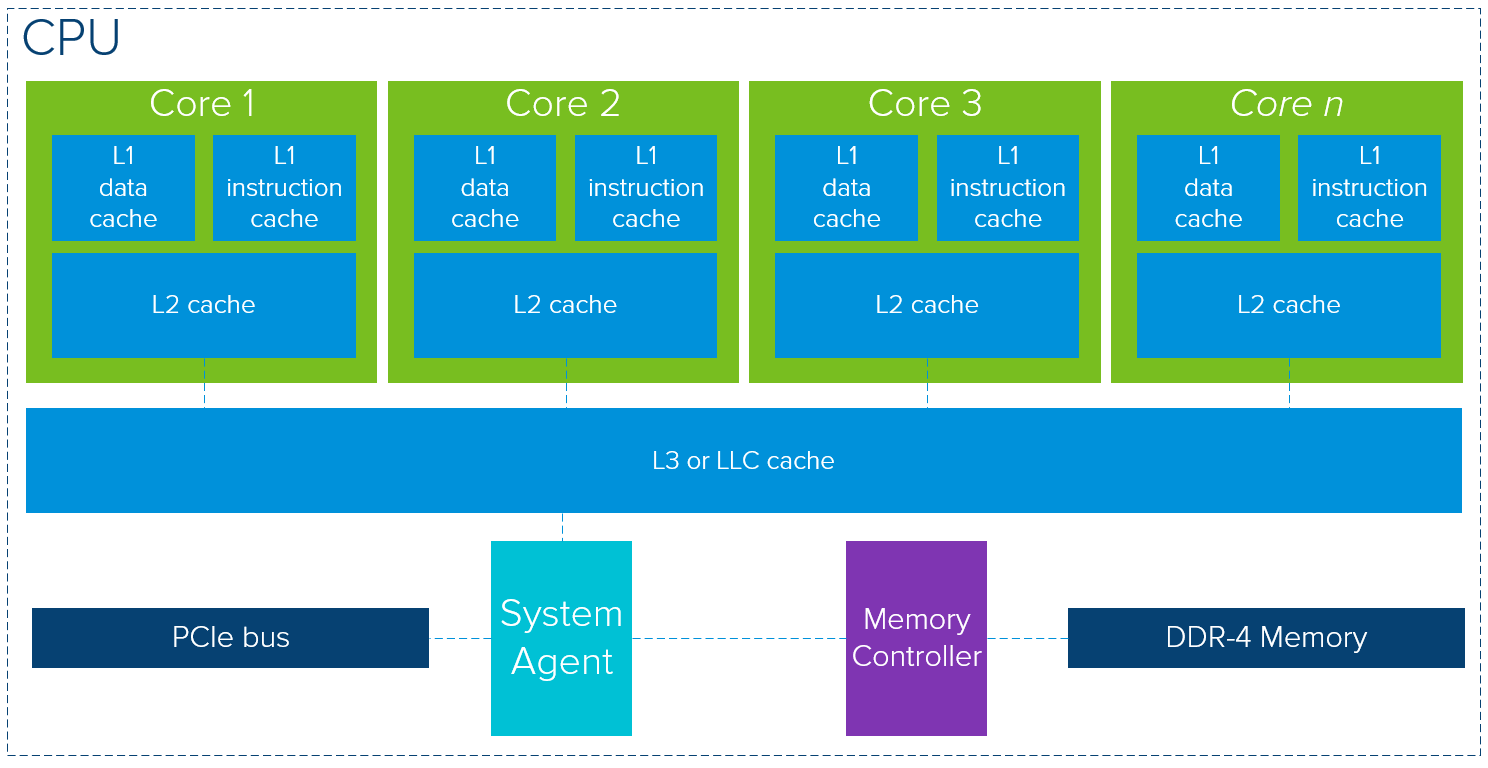
\includegraphics[width=0.75\textwidth]{./cpuArchitecture.png}
  \end{figure}
  \let\thefootnote\relax\footnotetext{https://core.vmware.com/resource/exploring-gpu-architecture}
\end{frame}
%%%%%%%%%%%%%%%%%%%%%%%%%%%%%%%%%%%%%%%%%%%%%%%%%%%%%%%%%%%%%%%%%%%%%%%%%%%%% 

%%%%%%%%%%%%%%%%%%%%%%%%%%%%%%%%%%%%%%%%%%%%%%%%%%%%%%%%%%%%%%%%%%%%%%%%%%%%% 
\begin{frame}[fragile]{Parallel paradigms: GPU}
  \begin{figure}
    \centering
    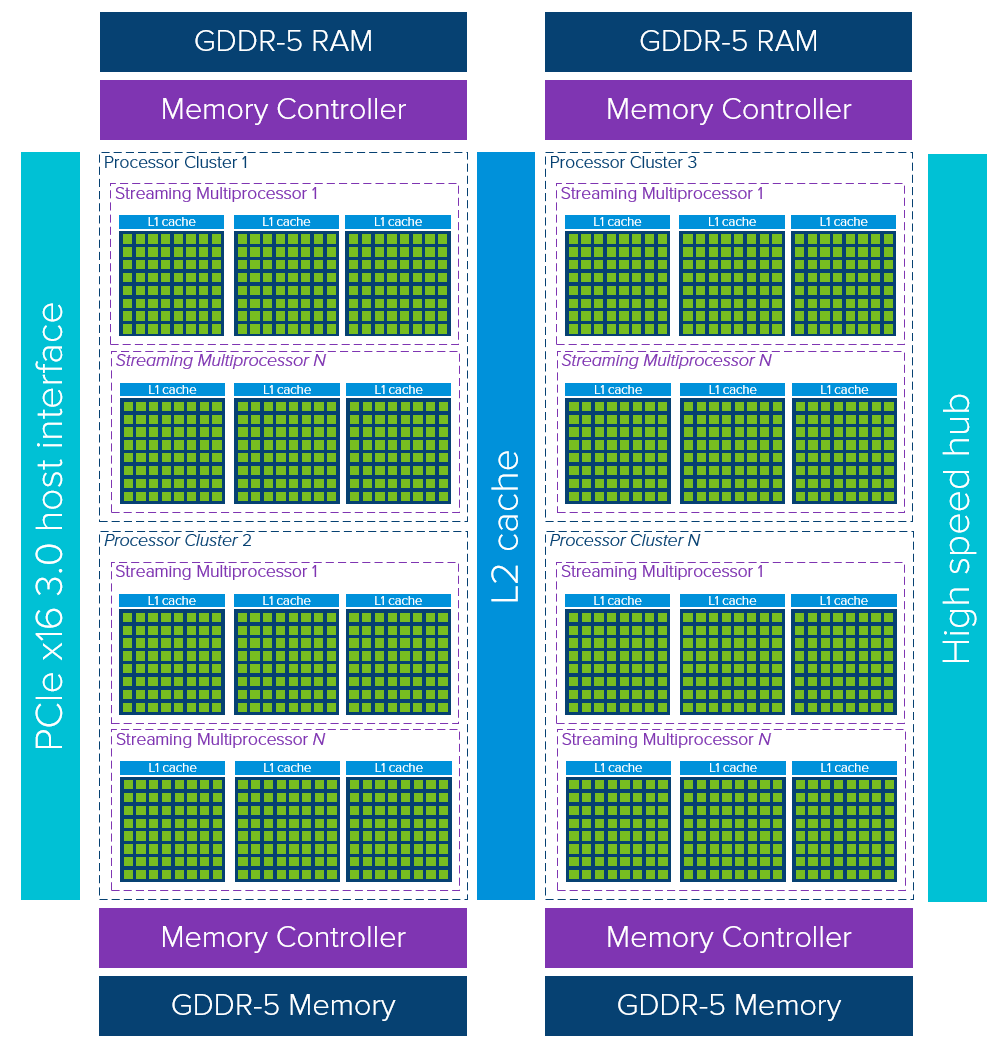
\includegraphics[width=0.6\textwidth]{./gpuArchitecture.png}
  \end{figure}
  \let\thefootnote\relax\footnotetext{https://core.vmware.com/resource/exploring-gpu-architecture}
\end{frame}
%%%%%%%%%%%%%%%%%%%%%%%%%%%%%%%%%%%%%%%%%%%%%%%%%%%%%%%%%%%%%%%%%%%%%%%%%%%%% 

%%%%%%%%%%%%%%%%%%%%%%%%%%%%%%%%%%%%%%%%%%%%%%%%%%%%%%%%%%%%%%%%%%%%%%%%%%%%% 
\begin{frame}[fragile]{Parallel paradigms: Multi-node}
  \begin{figure}
    \centering
    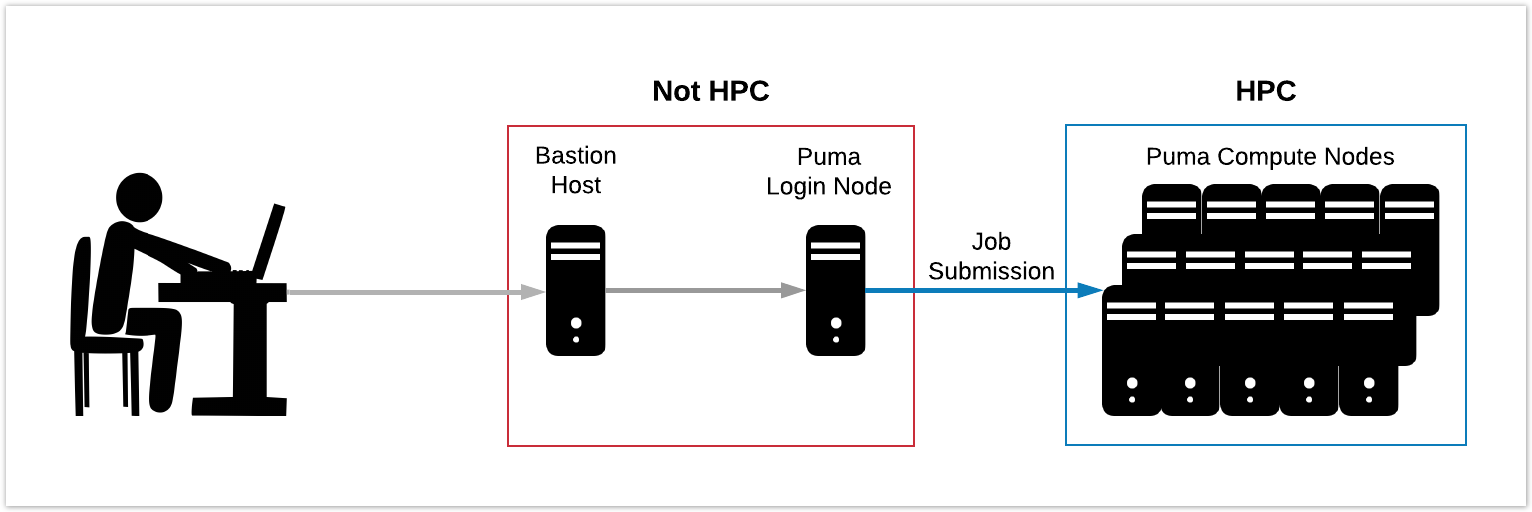
\includegraphics[width=0.75\textwidth]{./hpcArchitecture.png}
  \end{figure}
  \begin{figure}
    \centering
    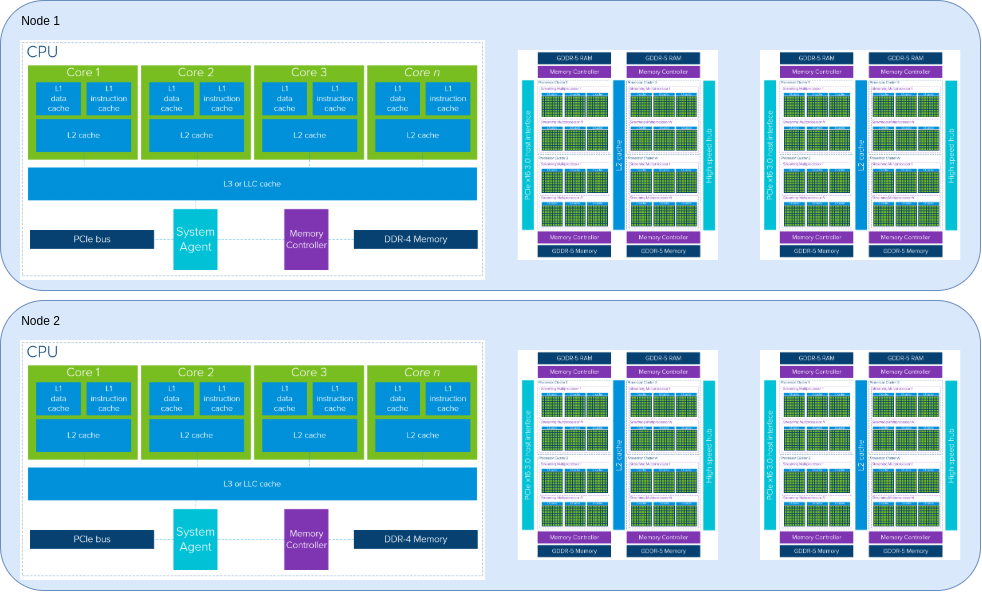
\includegraphics[width=0.6\textwidth]{./multi-node.png}
  \end{figure}
  \let\thefootnote\relax\footnotetext{https://public.confluence.arizona.edu/display/UAHPC/Puma+Quick+Start}
\end{frame}
%%%%%%%%%%%%%%%%%%%%%%%%%%%%%%%%%%%%%%%%%%%%%%%%%%%%%%%%%%%%%%%%%%%%%%%%%%%%% 

%%%%%%%%%%%%%%%%%%%%%%%%%%%%%%%%%%%%%%%%%%%%%%%%%%%%%%%%%%%%%%%%%%%%%%%%%%%%% 
\begin{frame}[fragile]{Word of warning}
  \begin{itemize}
  \item Not all code is parallelizable! Improper implementations can lead to
    \begin{itemize}
    \item Race conditions
    \item Deadlock
    \item Memory Corruption
    \end{itemize}
  \end{itemize}
  \verb+badParallel.jl+
  \verbatiminput{../src/badParallel.jl}

\end{frame}
%%%%%%%%%%%%%%%%%%%%%%%%%%%%%%%%%%%%%%%%%%%%%%%%%%%%%%%%%%%%%%%%%%%%%%%%%%%%% 

%%%%%%%%%%%%%%%%%%%%%%%%%%%%%%%%%%%%%%%%%%%%%%%%%%%%%%%%%%%%%%%%%%%%%%%%%%%%% 
\begin{frame}[t, fragile]{CPU Thread parallelism}
  \begin{columns}[t]
  \column{0.45\linewidth}
    Julia: \verb+helloWorld.jl+ \\
    ---------------------------------------------
    \small{
    \verbatiminput{../src/helloWorld.jl}}

  \column{0.45\linewidth}
    Python: \verb+helloWorld.py+ \\
    ---------------------------------------------
    \small{
      \verbatiminput{../src/helloWorld.py}}

  \end{columns}
\end{frame}
%%%%%%%%%%%%%%%%%%%%%%%%%%%%%%%%%%%%%%%%%%%%%%%%%%%%%%%%%%%%%%%%%%%%%%%%%%%%% 

%%%%%%%%%%%%%%%%%%%%%%%%%%%%%%%%%%%%%%%%%%%%%%%%%%%%%%%%%%%%%%%%%%%%%%%%%%%%% 
\begin{frame}{GPU Thread parallelism}
  \begin{itemize}
  \item \href{https://developer.nvidia.com/blog/even-easier-introduction-cuda/}{Even easier introduction to Cuda}
  \end{itemize}
\end{frame}
%%%%%%%%%%%%%%%%%%%%%%%%%%%%%%%%%%%%%%%%%%%%%%%%%%%%%%%%%%%%%%%%%%%%%%%%%%%%% 

%%%%%%%%%%%%%%%%%%%%%%%%%%%%%%%%%%%%%%%%%%%%%%%%%%%%%%%%%%%%%%%%%%%%%%%%%%%%% 
\begin{frame}[fragile]{Node parallelism via Slurm}
  \verb+monteCarlo.jl+ \\
  ---------------------------------------------
  \small{
    \verbatiminput{../src/nodeParallelism/monteCarlo.jl}}
\end{frame}
%%%%%%%%%%%%%%%%%%%%%%%%%%%%%%%%%%%%%%%%%%%%%%%%%%%%%%%%%%%%%%%%%%%%%%%%%%%%% 

%%%%%%%%%%%%%%%%%%%%%%%%%%%%%%%%%%%%%%%%%%%%%%%%%%%%%%%%%%%%%%%%%%%%%%%%%%%%%
\begin{frame}[fragile]{Node parallelism via Slurm}
  \tiny{
    \verb+monteCarlo.slurm+\\
    ---------------------------------------------
    \verbatiminput{../src/nodeParallelism/monteCarlo.slurm}}
\end{frame}
%%%%%%%%%%%%%%%%%%%%%%%%%%%%%%%%%%%%%%%%%%%%%%%%%%%%%%%%%%%%%%%%%%%%%%%%%%%%% 

%%%%%%%%%%%%%%%%%%%%%%%%%%%%%%%%%%%%%%%%%%%%%%%%%%%%%%%%%%%%%%%%%%%%%%%%%%%%% 
\begin{frame}{References \& Further Reading}
  \begin{small}
  \begin{itemize}
  \item \href{https://core.vmware.com/resource/exploring-gpu-architecture}{https://core.vmware.com/resource/exploring-gpu-architecture}
  \item \href{https://public.confluence.arizona.edu/display/UAHPC/Puma+Quick+Start}{https://public.confluence.arizona.edu/display/UAHPC/Puma+Quick+Start}
  \item \href{https://www.tensorflow.org/guide/gpu}{https://www.tensorflow.org/guide/gpu}
  \item \href{https://developer.nvidia.com/blog/even-easier-introduction-cuda/}{https://developer.nvidia.com/blog/even-easier-introduction-cuda/}
  \item \href{https://public.confluence.arizona.edu/display/UAHPC/Using+and+Installing+Python}{https://public.confluence.arizona.edu/display/UAHPC/Using+and+Installing+Python}
    
  \end{itemize}
  \end{small}
\end{frame}
%%%%%%%%%%%%%%%%%%%%%%%%%%%%%%%%%%%%%%%%%%%%%%%%%%%%%%%%%%%%%%%%%%%%%%%%%%%%% 

\end{document}